../cictikz/src/cictikz/data/tex/cictikz_preamble.tex

% Conduction band with V_D > 0: the drain side is pulled down by qV_D
% (dotted: the V_DS = 0 band), so injection from drain to bulk becomes
% improbable and a net electron current flows from source to drain.

\definecolor{regg}{RGB}{20,140,60}
\definecolor{lblred}{RGB}{225,60,45}
\definecolor{eblue}{RGB}{40,40,180}

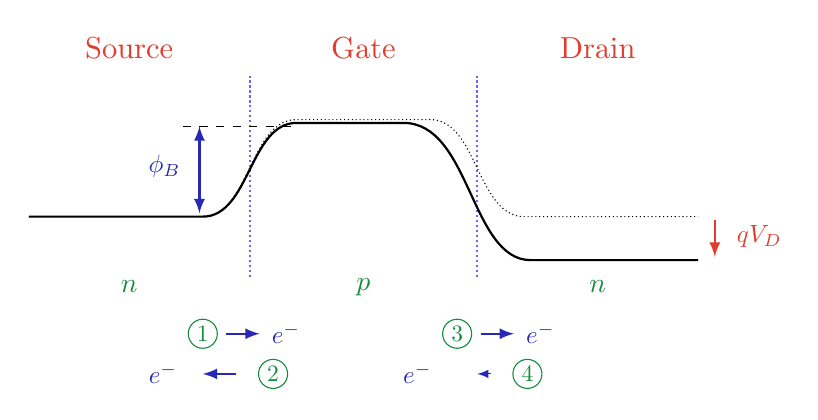
\begin{tikzpicture}[scale=0.85]

  \draw[densely dotted, thick, blue!60] (3.3,0.3) -- (3.3,3.3);
  \draw[densely dotted, thick, blue!60] (6.7,0.3) -- (6.7,3.3);

  % V_DS = 0 band for reference
  \draw[black, densely dotted]
    (0,1.2) -- (2.6,1.2) .. controls (3.3,1.2) and (3.3,2.65) .. (4.0,2.65)
    -- (6.0,2.65) .. controls (6.7,2.65) and (6.7,1.2) .. (7.4,1.2) -- (10,1.2);

  % band with the drain pulled down
  \draw[black, thick]
    (0,1.2) -- (2.6,1.2) .. controls (3.3,1.2) and (3.3,2.6) .. (4.0,2.6)
    -- (5.6,2.6) .. controls (6.6,2.6) and (6.6,0.55) .. (7.5,0.55) -- (10,0.55);

  % qV_D at the drain
  \draw[lblred, thick, -latex] (10.25,1.15) -- (10.25,0.6);
  \node[lblred, anchor=west, scale=0.9] at (10.45,0.9) {$qV_D$};

  % barrier height
  \draw[black, dashed, thin] (2.3,2.55) -- (4.0,2.55);
  \draw[eblue, thick, latex-latex] (2.55,1.25) -- (2.55,2.55);
  \node[eblue, anchor=east, scale=0.9] at (2.4,1.95) {$\phi_B$};

  % region labels
  \node[lblred, anchor=south, scale=1.1] at (1.5,3.4) {Source};
  \node[lblred, anchor=south, scale=1.1] at (5.0,3.4) {Gate};
  \node[lblred, anchor=south, scale=1.1] at (8.5,3.4) {Drain};
  \node[regg, anchor=center, scale=1.0] at (1.5,0.15) {$n$};
  \node[regg, anchor=center, scale=1.0] at (5.0,0.15) {$p$};
  \node[regg, anchor=center, scale=1.0] at (8.5,0.15) {$n$};

  % injection currents: 4 is now much smaller
  \node[regg, anchor=center, scale=0.85, circle, draw=regg, inner sep=1.5pt] at (2.6,-0.55) {1};
  \draw[eblue, thick, -latex] (2.95,-0.55) -- (3.45,-0.55);
  \node[eblue, anchor=west, scale=0.9] at (3.5,-0.55) {$e^-$};
  \node[eblue, anchor=east, scale=0.9] at (2.35,-1.15) {$e^-$};
  \draw[eblue, thick, -latex] (3.1,-1.15) -- (2.6,-1.15);
  \node[regg, anchor=center, scale=0.85, circle, draw=regg, inner sep=1.5pt] at (3.65,-1.15) {2};

  \node[regg, anchor=center, scale=0.85, circle, draw=regg, inner sep=1.5pt] at (6.4,-0.55) {3};
  \draw[eblue, thick, -latex] (6.75,-0.55) -- (7.25,-0.55);
  \node[eblue, anchor=west, scale=0.9] at (7.3,-0.55) {$e^-$};
  \node[eblue, anchor=east, scale=0.9] at (6.15,-1.15) {$e^-$};
  \draw[eblue, thin, -latex] (6.9,-1.15) -- (6.7,-1.15);
  \node[regg, anchor=center, scale=0.85, circle, draw=regg, inner sep=1.5pt] at (7.45,-1.15) {4};

\end{tikzpicture}
\end{document}
